%%%%%%%%%%%%%%%%%%%%%%%%%%%%%%%%%%%%%%%%%%%%%%%%%%%%%%%%%%%%%%%%%%%%%%%%%%%
%
% Template for a LaTex article in English.
%
%%%%%%%%%%%%%%%%%%%%%%%%%%%%%%%%%%%%%%%%%%%%%%%%%%%%%%%%%%%%%%%%%%%%%%%%%%%

\documentclass[12pt,a4paper]{article}
\usepackage{graphicx}
\usepackage[utf8]{inputenc}

% AMS packages:
\usepackage{amsmath, amsthm, amsfonts}

% Theorems
%-----------------------------------------------------------------
\newtheorem{thm}{Theorem}[section]
\newtheorem{cor}[thm]{Corollary}
\newtheorem{lem}[thm]{Lemma}
\newtheorem{prop}[thm]{Proposition}
\theoremstyle{definition}
\newtheorem{defn}[thm]{Definition}
\theoremstyle{remark}
\newtheorem{rem}[thm]{Remark}

% Shortcuts.
% One can define new commands to shorten frequently used
% constructions. As an example, this defines the R and Z used
% for the real and integer numbers.
%-----------------------------------------------------------------
\def\RR{\mathbb{R}}
\def\ZZ{\mathbb{Z}}

% Similarly, one can define commands that take arguments. In this
% example we define a command for the absolute value.
% -----------------------------------------------------------------
\newcommand{\abs}[1]{\left\vert#1\right\vert}

% Operators
% New operators must defined as such to have them typeset
% correctly. As an example we define the Jacobian:
% -----------------------------------------------------------------
\DeclareMathOperator{\Jac}{Jac}

%-----------------------------------------------------------------
\title{Template for a \LaTeX\ article}
\author{Angela Menéndez\\
  \small Dept. Templates and Editors\\
  \small E12345\\
  \small Spain
}

\begin{document}
\maketitle

\abstract{This is a simple template for an article written in \LaTeX.}

\section{First section}

Here goes the text.
\begin{equation}\label{eq:area}
  S = \pi r^2
\end{equation}
\[S_n = \sum_{n=1}^{\infty} \frac{1}{n^3} + \sum_{n=1}^{\infty} \frac{1}{n^3}\] 

One can refer to equations like this: see equation (\ref{eq:area}). One can also
refer to sections in the same way: see section \ref{sec:nothing}. Or
to the bibliography like this: \cite{Cd94}.

\subsection{Subsection}\label{sec:nothing}

More text. Claro 
\[\RR\]
\[\ZZ\]

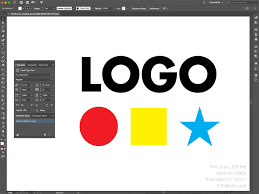
\includegraphics[width=0.8\textwidth]{./figs/drawing.png}

\subsubsection{Subsubsection}\label{sec:nothing2}

More text

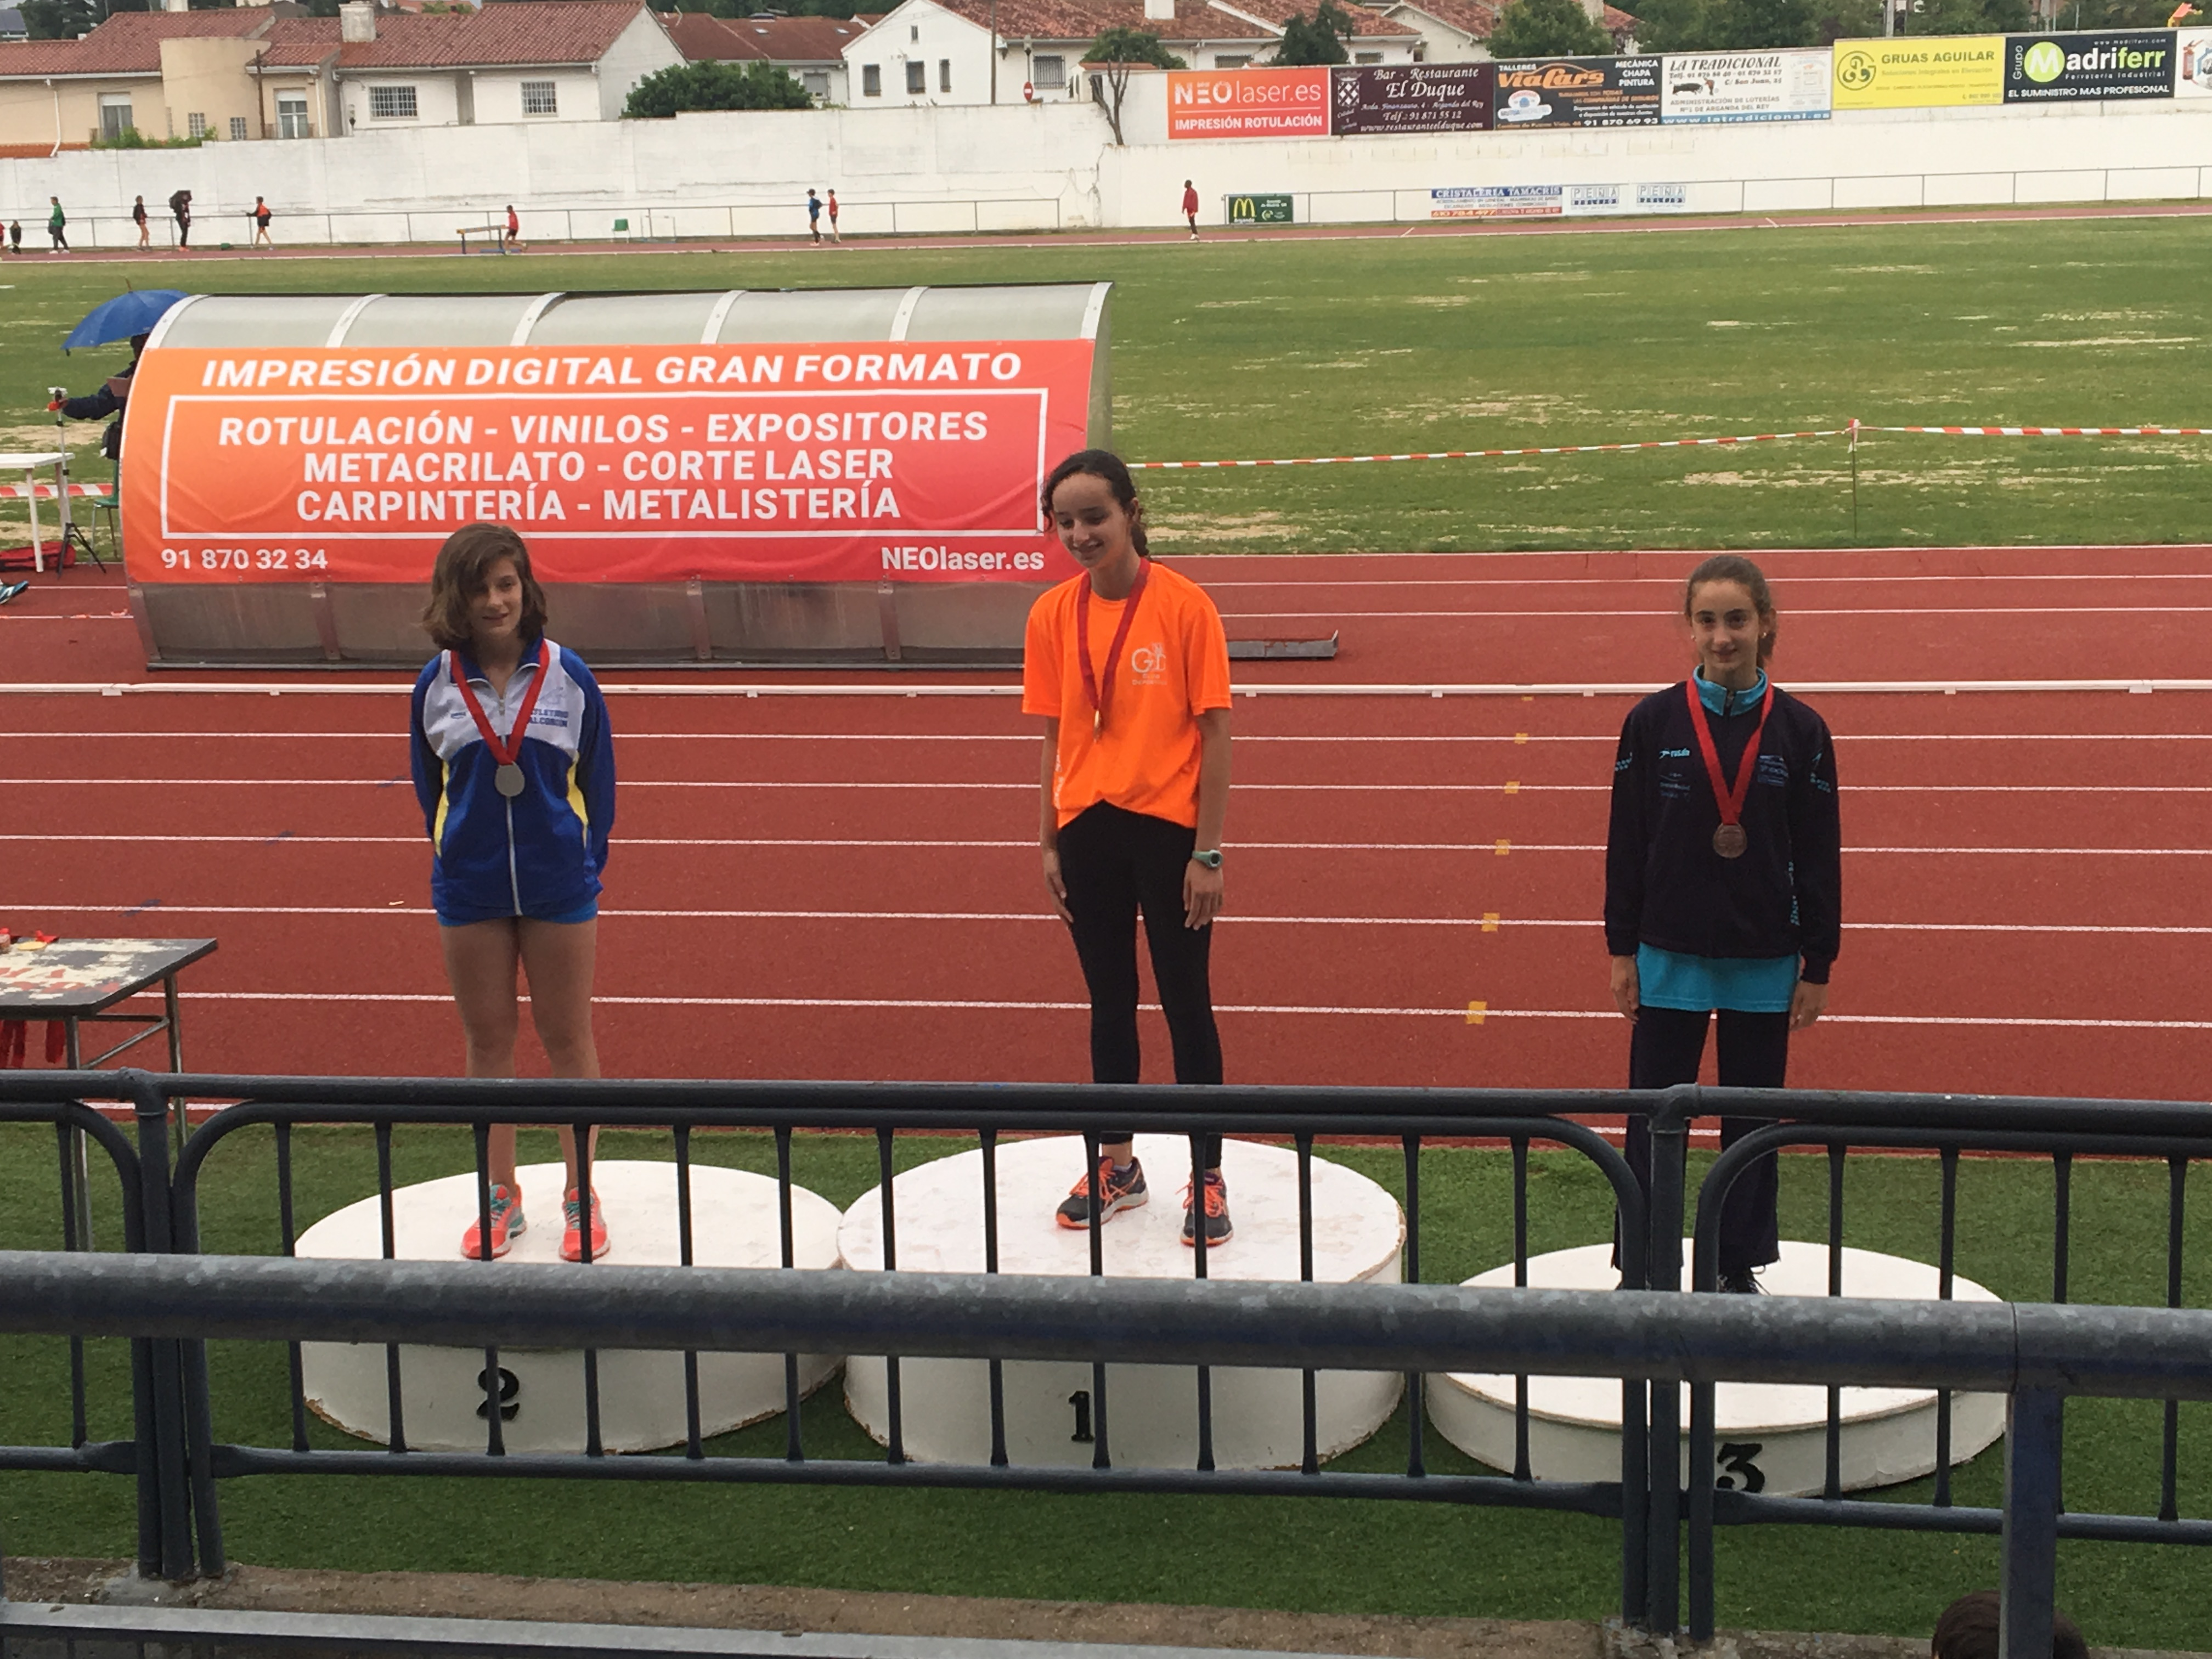
\includegraphics[width=0.8\textwidth]{./figs/picture.JPG}


% Bibliography
%-----------------------------------------------------------------
\begin{thebibliography}{99}

\bibitem{Cd94} Author, \emph{Title}, Journal/Editor, (year)

\end{thebibliography}


\end{document}
